\documentclass[12pt]{article}
\usepackage[paper=letterpaper,margin=2cm]{geometry}
\usepackage{amsmath}
\usepackage{amssymb}
\usepackage{amsfonts}
\usepackage{newtxtext, newtxmath}
\usepackage{enumitem}
\usepackage{titling}
\usepackage[colorlinks=true]{hyperref}
\usepackage{graphicx}
\usepackage{float}
\usepackage{listings}
\usepackage{xcolor}
\lstset{
    numbers=left, 
    numberstyle= \tiny, 
    keywordstyle= \color{ blue!70},
    commentstyle= \color{red!50!green!50!blue!50}, 
    frame=shadowbox, % 阴影效果
    rulesepcolor= \color{ red!20!green!20!blue!20} ,
    escapeinside=``, % 英文分号中可写入中文
    xleftmargin=2em,xrightmargin=2em, aboveskip=1em,
    framexleftmargin=2em
} 

\setlength{\droptitle}{-6em}

% Enter the specific assignment number and topic of that assignment below, and replace "Your Name" with your actual name.
\title{Assignment 1: Comp 6771 Image Processing}
\author{Yunqi Xu 40130514}
\date{\today}



\begin{document}
% \maketitle

\begin{titlepage}
  \rule{\textwidth}{1pt}   % The top horizontal rule
    \vspace{0.2\textheight}  % Whitespace between top horizontal rule and title

    %------------------------------------------------------------
    %    Title
    %------------------------------------------------------------

    {\Huge COMP 6771 Image Processing: Assignment 1}

    \vspace{0.025\textheight}   % Whitespace between the title and short horizontal rule

    \rule{0.83\textwidth}{0.4pt}  % The short horizontal rule under title

    \vspace{0.1\textheight}  % Whitespace between the short horizontal rule and author

    %------------------------------------------------------------
    %    Author
    %------------------------------------------------------------

    {\Large Student name: \textsc{Yunqi Xu}}
    \vfill
    {\Large Student id: 40130514}
    \vfill  % Whitespace between author and date

    {\large \today}
    \vspace{0.1\textheight}  % Whitespace between date and bottom horizontal rule

    %------------------------------------------------------------
    %    Bottom rules
    %------------------------------------------------------------

    \rule{\textwidth}{1pt}  % The bottom horizontal rule
\end{titlepage}

\begin{enumerate}[leftmargin=\labelsep]
% \vspace*{40em}
\item Question 1
    \begin{enumerate}
    \item  Explain why the discrete histogram equalization technique does not, in general, yield a flat histogram.
    \vspace*{1em}
    If we want a flat histogram, we need to guarantee each component has the same pixels in it. 
    Let's set $n$ be the total number of pixels, and $L$ be the intensity levels. 
    The flat histogram will require each component has $n/L$ number of pixels. 
    However, the Histogram Equalization process will re-mapping the pixels only based on their intensity level.
    So, we can not control the number of pixels in each conponent, it is difficult to yield a flat histogra. 
    
    \item Suppose that a digital image is subjected to histogram equalization. Please elaborate why a second pass of histogram equalization (on the histogram-equalized image) will produce exactly the same result as the first pass.
    \vspace*{1em}
    Suppose an image has already pass a histogram equalization. 
    Input this image into the second second pass of histogram equalization. 
    Let $n$ is the total number of pixels, and $L$ is the intensity level.

        $$
        s_k = T(r_k) = (L-1)\sum{j=0}^k n_{rj}/n = \frac{L-1}{n} \sum_{j=0}^k n_{rj} = (L-1)\sum_{j = 0}^k p_r(rj)
        $$
        we will use the equation mentioned above to calculate the $s_k$.
        Since every pixel belong to $r_k$ is distributed to $s_k$.
        So, the $n_{sk}$ = $n_{rk}$
        $$
        p_s(s_k) = n_{sk} / n = n_{rk} / n = p_r(r_k)
        $$
        Also, no matter how many iterations,
        $$
        new_k = (L-1)\sum_{j=0}^k p_s(s_k) = (L-1)\sum_{j=0}^k p_r(r_k) = s_k
        $$
        Therefore, the second pass will get the same result as the first pass. 

    \end{enumerate}


\item Given two arbitrary images f(x,y) and g(x,y) and two arbitrary constant a and b, H is said to be a linear operator if:
$$
        H[af(x, y) + bg(x, y)] = aH[f(x,y) + bH[g(x,y)]]
$$
The median m of a set of numbers is such that half the values in the set are below m and the other half are above it (the mid-point value by population). Is an operator that computes the median of a set of pixels of a sub-image area linear or nonlinear? Explain your answer by giving examples.

\vspace*{1em}
In general, the median operator is not linear operator.
Since we can not control the order of values in $f(x,y)$ or $g(x,y)$.
We will re-order the values in $f(x,y)$ and $g(x,y)$ and the the result of $af(x,y) + bg(x,y)$ before we get the median value.

In some specific case, median operator will be linear, for example, if the the median value located in the center of $f(x,y)$ and $g(x,y)$ and the value in the left are smaller or equal then the median and the values in the right are greater or equal than the median in both $f(x,y)$ and $g(x,y)$, and after $af(x,y) + bg(x,y)$ the result still folloing the rules mentioned above, H will be a linear operator.

For example, suppose $f(x,y) = [1, -3, 5, 7, 9]$ and $g(x,y) = [2,4,6,8,10]$ and $a = 2$, $b = 3$. 
        \begin{equation}
        \begin{aligned}
        H[af(x,y) + bg(x,y)]
        &= H[[2, -6, 10, 14, 18] + [6, 12, 18, 24, 30]]\\
        &= H[8, 6, 28, 38, 48]\\
        &= 28
        \label{q2_1}
        \end{aligned}
        \end{equation}
        
        \begin{equation}
        \begin{aligned}
        aH[f(x,y)] + bH[g(x,y)]
        &= 2*H[5] + 3*H[6]\\
        &= 10 + 18\\
        &= 28
        \label{q2_2}
        \end{aligned}
        \end{equation}
Therefore, we can find that the Eq.~\ref{q2_1} $=$ Eq.~\ref{q2_2}.        

On the other hand, If the values in $f(x,y)$ and $g(x,y)$ not following the rules mentioned about, the H is not a linear operator.

For example, Let us set $f(x,y) = [1, 3, -5, 7, 9]$ and $g(x,y) = [2, 4, 6, 8 10]$, also, $a = 2$, $b = 3$.
        \begin{equation}
        \begin{aligned}
        H[af(x,y) + bg(x,y)]
        &= H[[2, 6, -10, 14, 18] + [6, 12, 18, 24, 30]]\\
        &= H[8, 18, 8, 38,48]\\
        &= 18
        \label{q2_3}
        \end{aligned}
        \end{equation}
        
        \begin{equation}
        \begin{aligned}
        aH[f(x,y)] + bH[g(x,y)]
        &= 2*H[3] + 3*H[6]\\
        &= 6 + 18\\
        &= 24
        \label{q2_4}
        \end{aligned}
        \end{equation}
Therefore, the Eq.~\ref{q2_3} $\neq$ Eq.~\ref{q2_4}.


\item  The purpose of this question is to perform histogram equalization to a given histogram and plot the resulting histogram. Given the following histogram where GL is Gray level, and NP is Number of pixels:
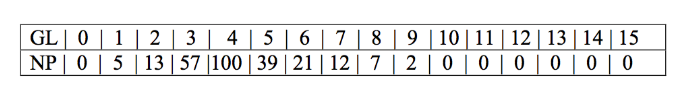
\includegraphics[]{Figure/Q3.Table_1.png}

        \begin{enumerate}
                \item Plot the histogram of the image given in the table above
                        \begin{figure}[H]
                        \centering
                        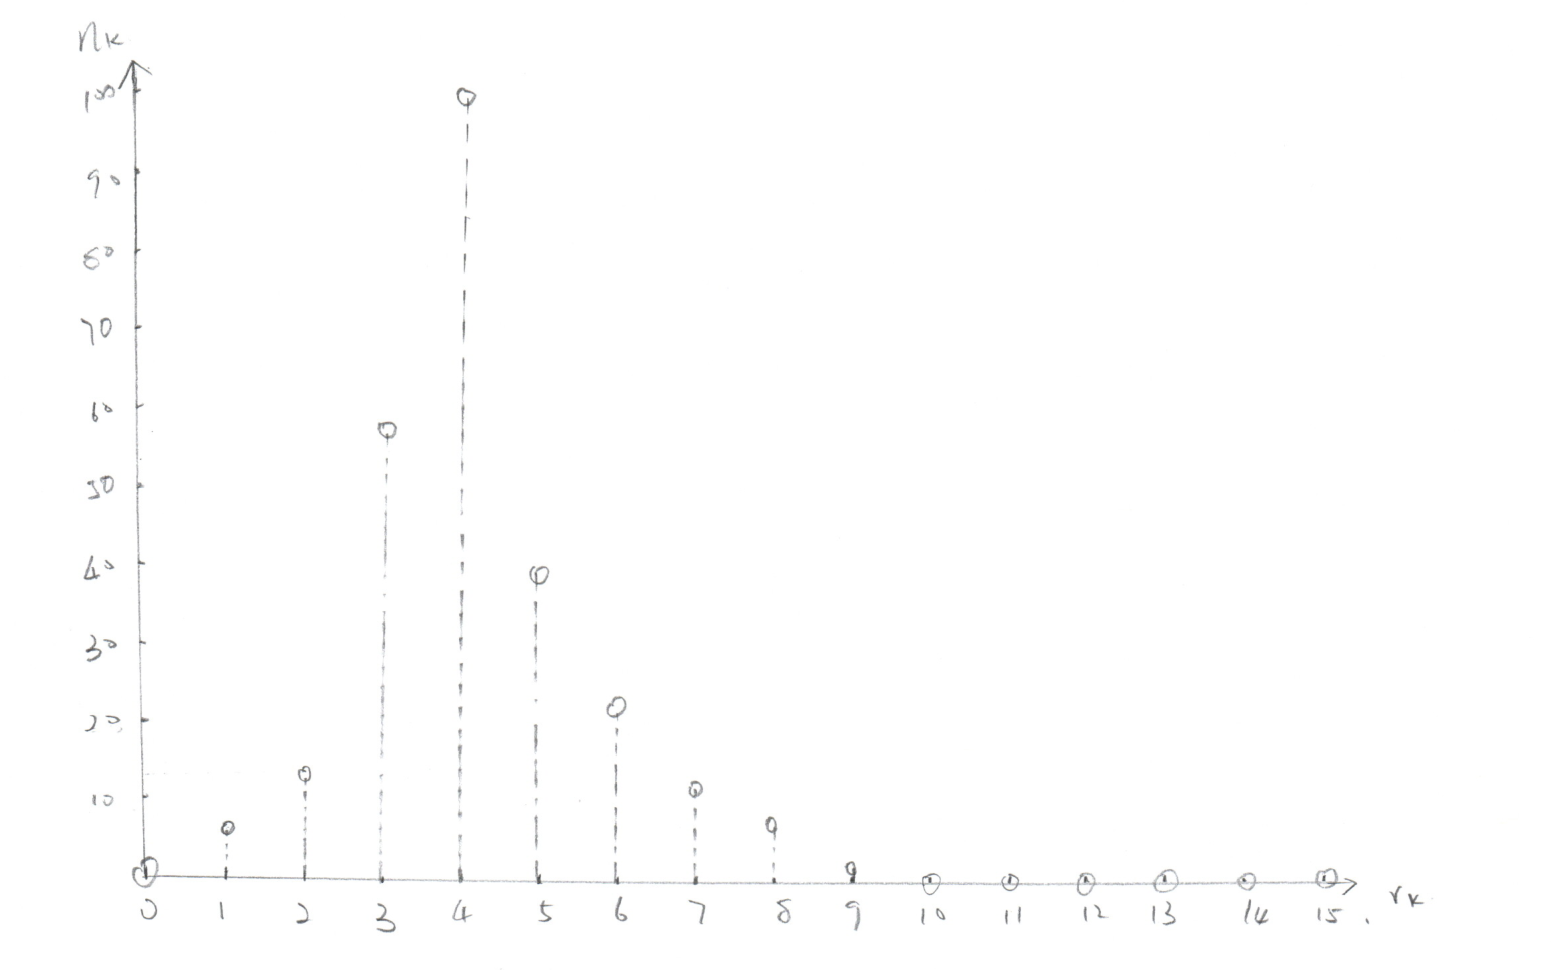
\includegraphics[]{Figure/Q3_a.png}
                        \caption{Histogram image}
                        \label{q3_a}
                        \end{figure}
                The Fig.~\ref{q3_a} presents the histogram based on the given table.
                \begin{enumerate}
                        \item Calculate sk from the table
                        \begin{figure}[H]
                        \centering
                        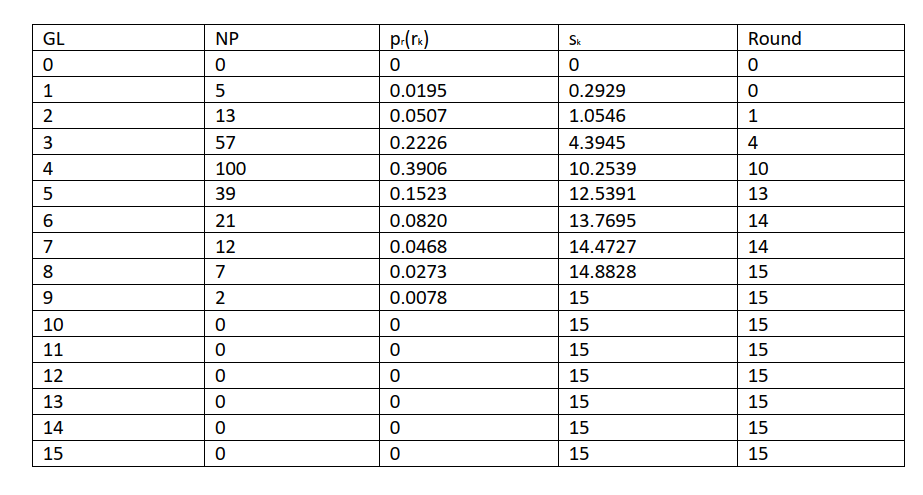
\includegraphics[]{Figure/Q3_b_1.png}
                        \caption{Calculation result}
                        \label{q3_b_1}
                        \end{figure}
                        The Fig.~\ref{q3_b_1} shows the calculation result of $s_k$. 
                        In This Figure, Let GL be the Gray Level $r_k$, and $NP$ is the number of pixels with value $r_k$, we will use $n_k$ later. Based on the given table, the total pixel $n = 256$, and $L = 15$
                        \begin{equation}
                                p_r(r_k) = \frac{n_k}{n} 
                        \label{eq_q3_b_1}
                        \end{equation}
                        \begin{equation}
                                s_k = \frac{L-1}{n}\sum_{j = 0}^k n_j
                        \label{eq_q3_b_2}
                        \end{equation}
                        And in the Fig.~\ref{q3_b_1}, we utilize the Eq.~\ref{eq_q3_b_1} and Eq.~\ref{eq_q3_b_2} to calcuation the $p_r(r_k)$ and $s_k$ respectively.
                \end{enumerate}
                \vspace*{2em}

                \item Plot the probability density functions pr (rk) and ps (sk)
                \begin{figure}[H]
                \centering
                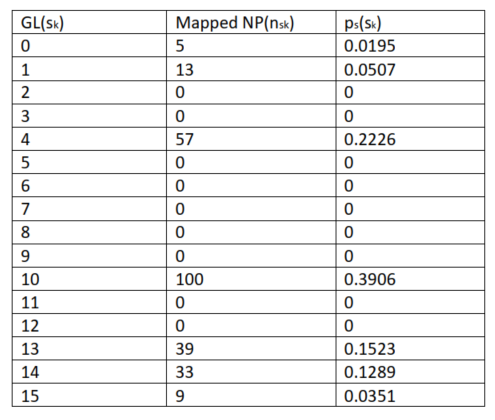
\includegraphics[]{Figure/Q3_b_2.png}
                \caption{Calculation of ps(sk)}
                \label{q3_b_2}
                \end{figure}
                We following the Histogram Equalization process to calculate those values in Fig.~\ref{q3_b_2}.

                \begin{figure}[H]
                \centering
                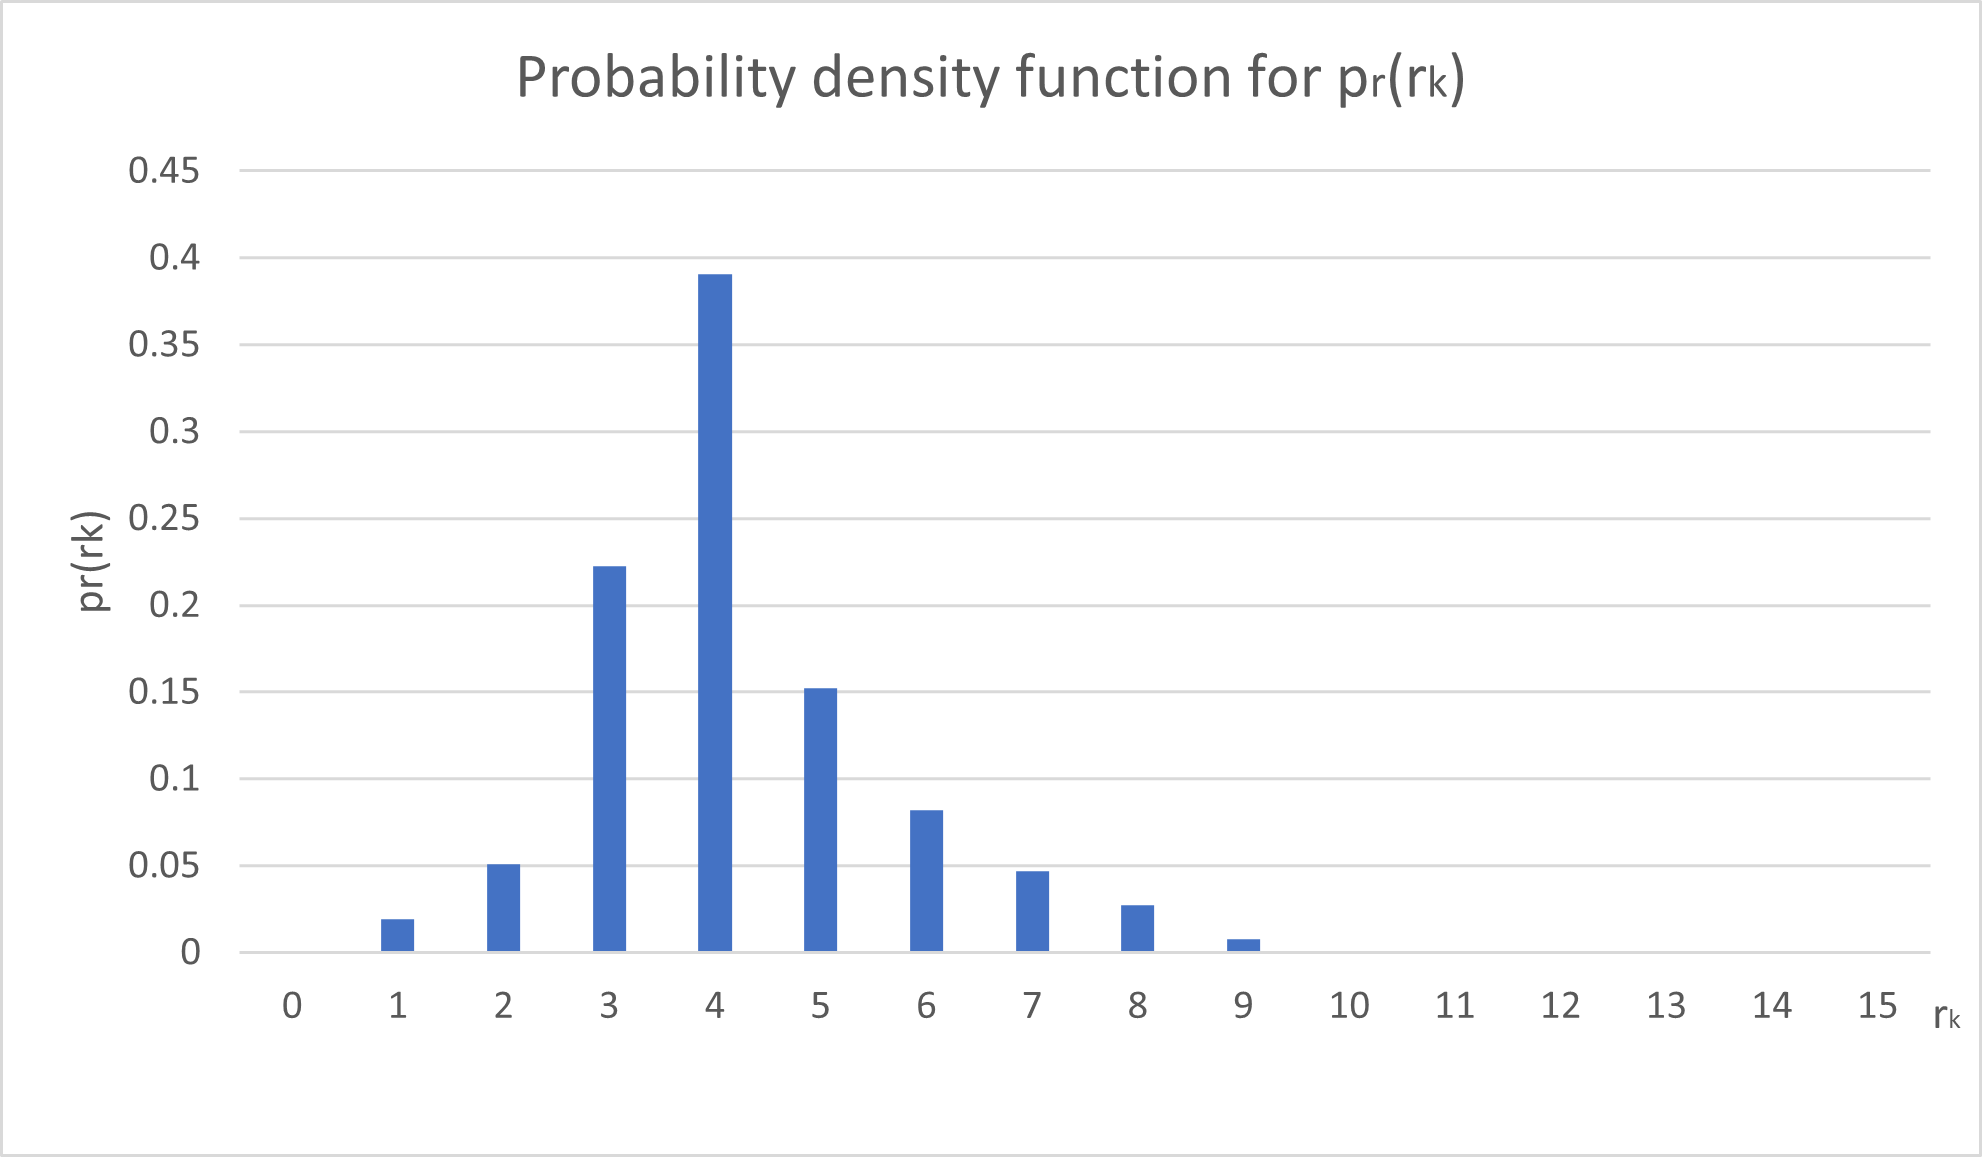
\includegraphics[]{Figure/q3_pr.png}
                \caption{Probability densi function for pr(rk)}
                \label{q3_pr}
                \end{figure}
                \begin{figure}[H]
                \centering
                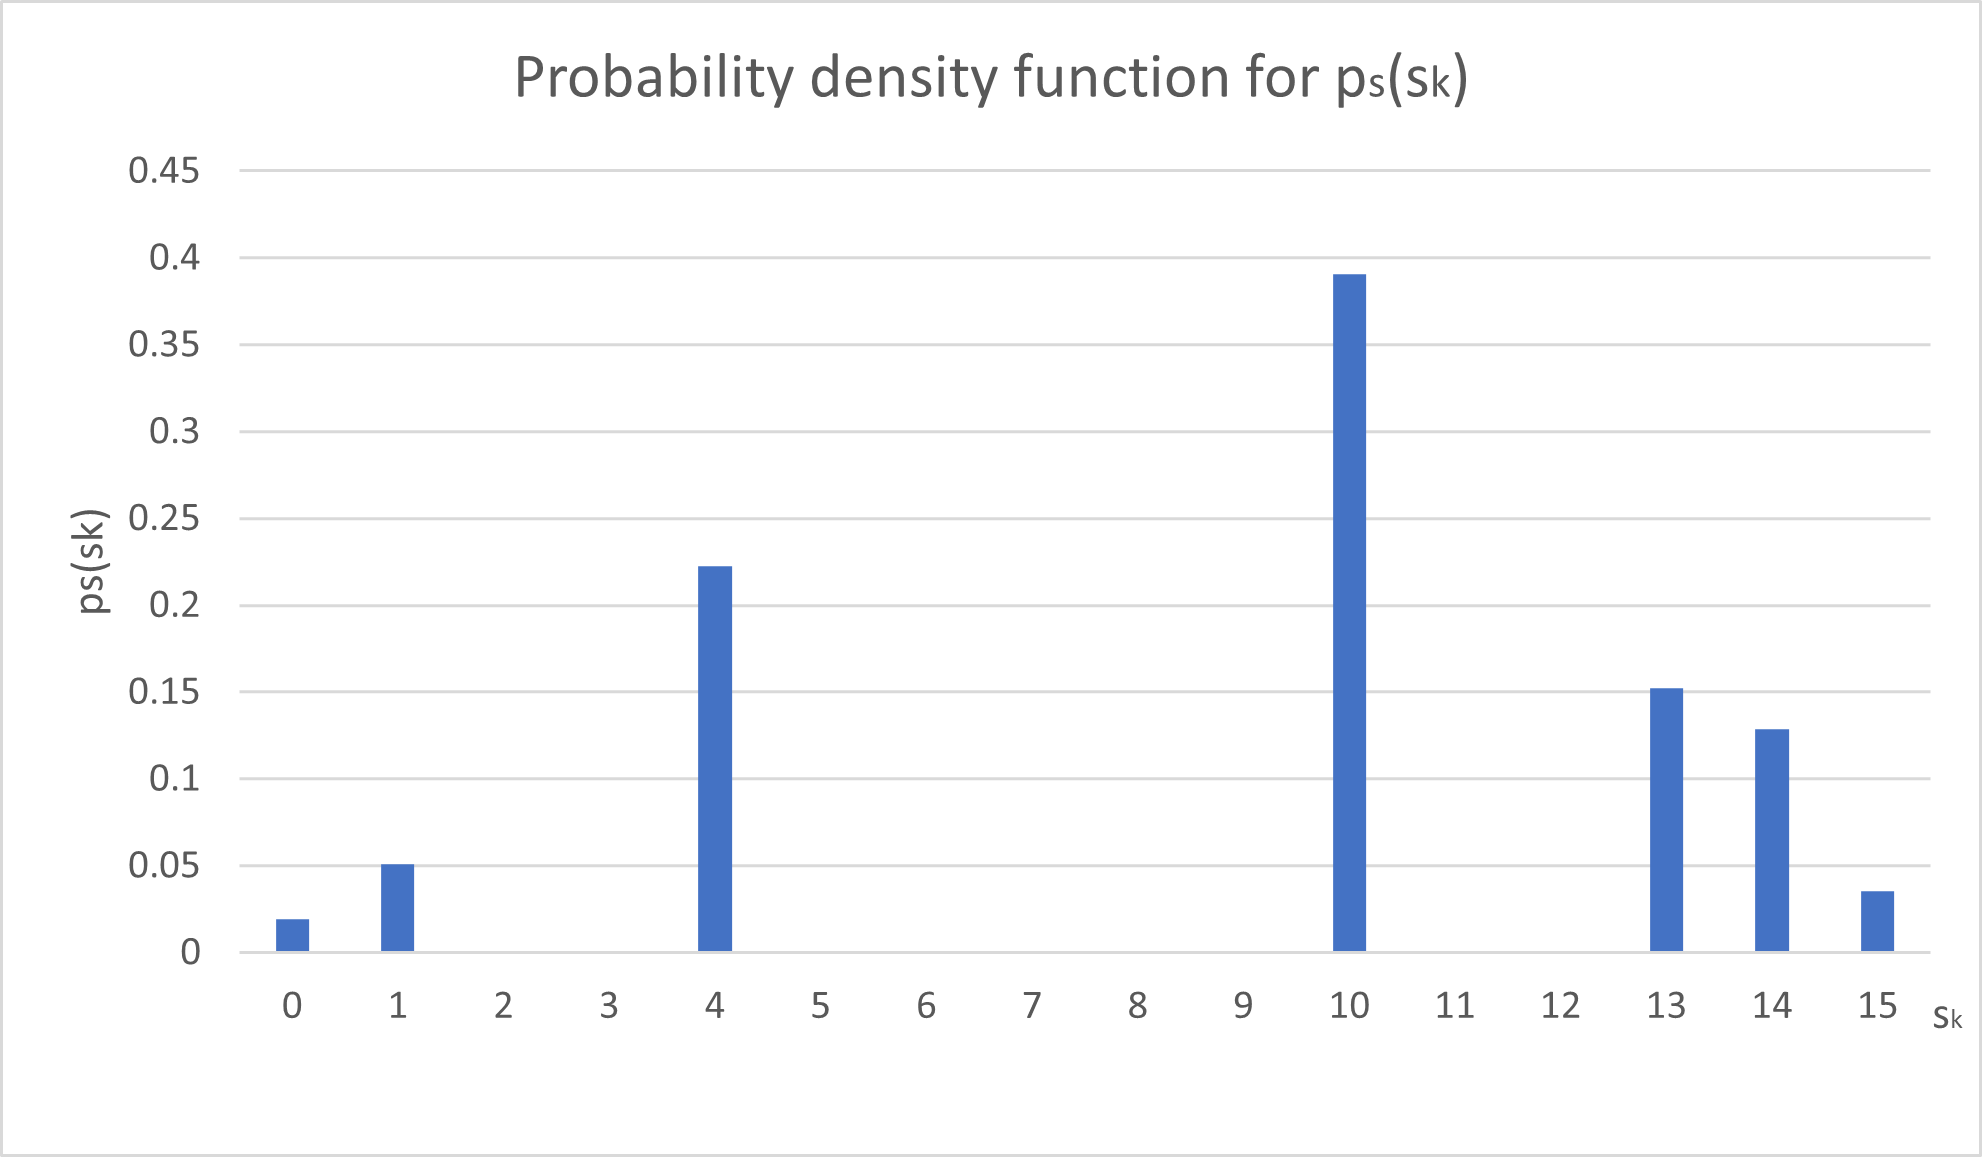
\includegraphics[]{Figure/q3_ps.png}
                \caption{Probability density function for ps(sk)}
                \label{q3_ps}
                \end{figure}
                Finally, we will get two probability density function present in Fig.~\ref{q3_pr} and Fig.~\ref{q3_ps}.

                \item Plot the new histogram after performing the histogram equalization.
                
                \begin{figure}[H]
                \centering
                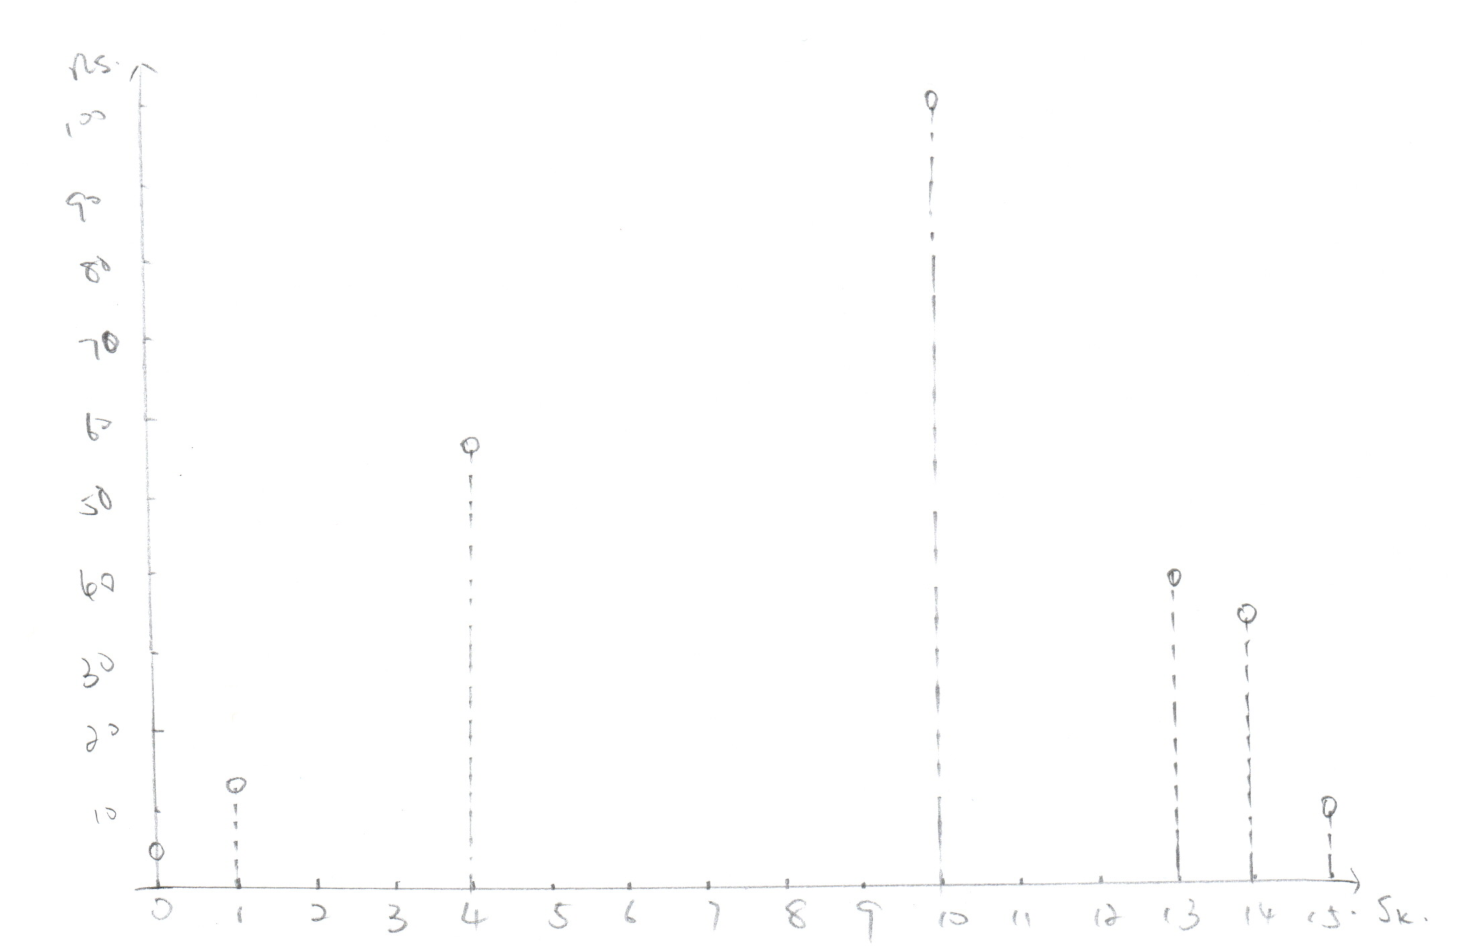
\includegraphics[]{Figure/q3_d.png}
                \caption{New histogram after histogram equalization}
                \label{q3_d}
                \end{figure}
                
                The new histogram is presented in Fig.~\ref{q3_d}.
                
        \end{enumerate}


\item The Given two images f(x,y) and g(x,y) with histogram hf and hg . Assuming that all the pixels of image g(x,y) have the same intensity equal to a non-zero positive constant value c. The gray levels of the pixels of both images have positive values. Please explain the relationship between the histograms of f(x,y) and the new images formed by f(x,y) + g(x,y) and f(x,y)*g(x,y)

\begin{enumerate}
        \item Since all the pixels of image $g(x,y)$ have the same intensity equal to a non-zero positive constant value $c$. 
        Set, $n(r_k)$ be the number of pixels belong to the intensity level $r_k$, then, the $f(x,y) + g(x,y) = f(x,y) + c$, So, the $n(r_k)$ will not change, but $r_k' = r_k + c$. 
        So, the histogram of new image $f(x,y)+g(x,y)$ will have the same hight as the histogram of $f(x,y)$ but all components will move to right with c.
        \item As mentioned above, t$f(x,y) * g(x,y) = f(x,y) * c$, So the hight will not change after the product operator, but the distance beteen each conponent will be enlarged by c, as $r_k' = r_k * c$. 
        For example, $r_k = 1$ will go to $r_k = c$ and $r_k = 2$ will go to $r_k = 2c$, $r_k = 3$ will go to $r_k = 3c$ ...
\end{enumerate}

\item Download the image from the assignment folder, and perform the following operations using MATLAB or any software packages you are familiar with. Please show your steps in the report.
\begin{lstlisting}
import numpy as np
import cv2
from matplotlib import pyplot as plt
\end{lstlisting}

        \begin{enumerate}
                \item Write a program to read the grayscales of the image.
\begin{lstlisting}
def read_grayscales(img):
        img = cv2.imread(img,0)
        return img
img_name = 'HawkesBay.jpeg'
img = read_grayscales(img_name)
\end{lstlisting}
                \item Write a program to calculate the histogram of the image and display the histogram chart.
\begin{lstlisting}
def calculate_histogram(img, L):
    image_flatten = img.flatten()
    new_list = np.zeros(L)
    for each_pixel in image_flatten:
        new_list[each_pixel] += 1
    return new_list 
        
def histogram_show(hist):
    plt.bar(range(len(hist)), hist)
    plt.xlabel("rk")
    plt.ylabel("nk")
    plt.title("Histogram of imput image")
    plt.savefig("Histogram_input")

histogram_statis = calculate_histogram(img, 256)
histogram_show(histogram_statis)
\end{lstlisting}
                The histogram is presented in Fig.\ref{q5_hist_input}.
                \begin{figure}[H]
                \centering
                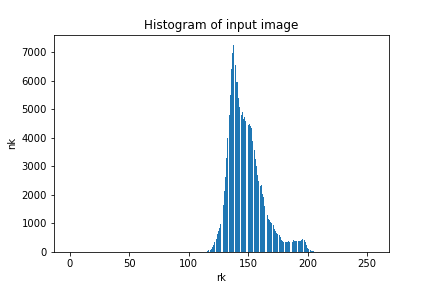
\includegraphics[]{Figure/Histogram_input.png}
                \caption{Histogram of input image}
                \label{q5_hist_input}
                \end{figure}
        

                \item Compare the calculated histogram obtained by using your own program with the one using the imhist function in MATLAB.
\begin{lstlisting}
img = imread("HawkesBay.jpeg")
imhist(img,256)
\end{lstlisting}
                The histogram from Matlab imhist function is present as Fig.~\ref{q5_hist_matlab}
                \begin{figure}[H]
                \centering
                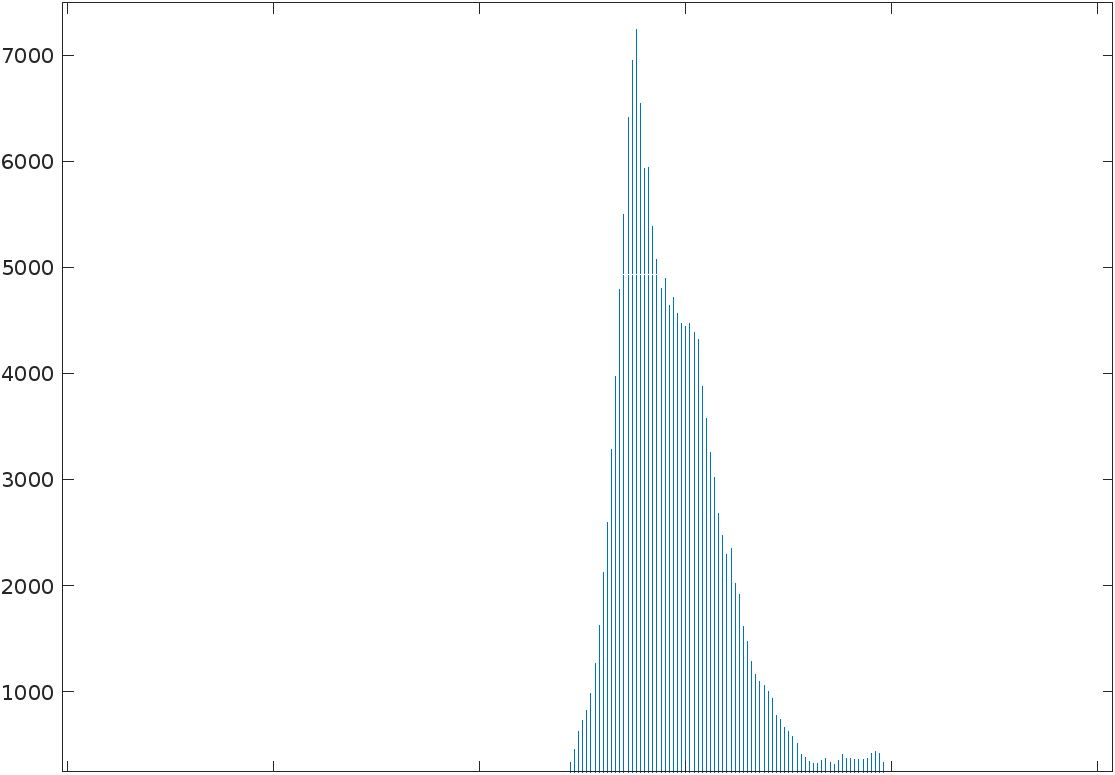
\includegraphics[]{Figure/hist_matlab.png}
                \caption{Histogram of Matlab imhist function}
                \label{q5_hist_matlab}
                \end{figure}

                \item Write a program to do histogram equalization on this image.
\begin{lstlisting}
def calculate_prob(hist,total_pixels):
    return [values_each_bin/total_pixels for values_each_bin in hist]

def calculate_sk(cal_pr, L):
    new_list = np.zeros(L)
    for index, each_pr in enumerate(cal_pr):
        cal_result = (L-1) * sum(cal_pr[0: index+1])
        new_list[index] = round(cal_result)
    return new_list

def new_image(img, sk):
    height, width = img.shape
    new_img = np.zeros(img.shape, dtype = 'uint8')
    for i in range(img.shape[0]):
        for j in range(img.shape[1]):
            new_img[i, j] = sk[img[i,j]]
    return new_img
tp = img.shape[0]*img.shape[1]
pr = calculate_prob(histogram_statis, tp)
sk = calculate_sk(pr, 256)
new_img = new_image(img, sk)
\end{lstlisting}

                \item Compare the histogram-equalized image obtained by using your own program with the one by using histeq function in MATLAB.
\begin{lstlisting}
J = histeq(I,256)
imshow(J)
\end{lstlisting}
                The new image from matlet histeq function is presented in Fig.~\ref{q5_matlab_newimage}
                \begin{figure}[H]
                \centering
                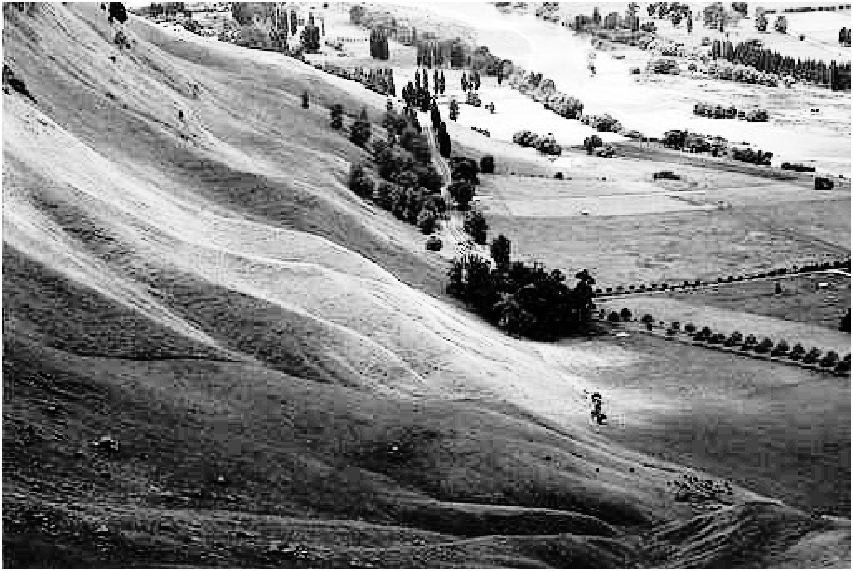
\includegraphics[width=0.8\textwidth,height=0.5\textwidth]{Figure/he_matlab_newimage.png}
                \caption{Histogram-equalized image obtained by Matlab histeq}
                \label{q5_matlab_newimage}
                \end{figure}
\begin{lstlisting}
cv2.imwrite("he_newimage.png",new_img)
\end{lstlisting}
                The new image from the histogram equalization problem is shown in Fig.~\ref{q5_python_newimage}
                \begin{figure}[H]
                \centering
                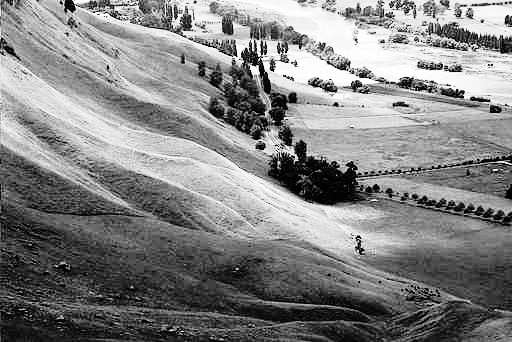
\includegraphics[width=0.8\textwidth,height=0.5\textwidth]{Figure/he_newimage.png}
                \caption{"histogram-equalized image obtained by my own program"}
                \label{q5_python_newimage}
                \end{figure}
                This two histogram-equalized images are very similar. 

                
        \end{enumerate}
\end{enumerate}

\end{document}
